\section{TEORIA DE RESPOSTA AO ITEM}
	\subsection{Introdução}
	\paragraph{}
	    A busca por informações de medidas de propriedades psicológicas dos indivíduos levou muitos pesquisadores a desenvolver modelos que pudessem estimar essas tais propriedades psicológicas, também referidas por traço latente, que são características individuais que não podem ser observadas diretamente, como por exemplo habilidade/proficiência em determinado conteúdo na avaliação educacional, atitude em relação à mudança organizacional, nível de ansiedade, nível de estresse, nível de depressão, qualidade de vida etc.).\textcite{Araujo}
	\par
		De acordo com \textcite{Dalton}, a Teoria da Resposta ao Item (TRI) é uma metodologia que sugere formas de representar a relação entre a probabilidade de um indivíduo dar uma resposta correta a um item, ver figura(\ref{fig:ques}) e seus traços latentes. Entretanto a TRI teve seus primórdios com a Teoria Clássica dos Testes(TCT). O presente trabalho não aborda todas os modelos da TRI e não busca esgotar o tema, pois trata-se de um tema muito complexo, teórico-matematicamente, e tem por objetivo mostrar a sua viabilidade para pesquisadores e seu uso mais difundido.
	\par
		Os teste e questionários são os principais agentes responsáveis pela coleta de informações, assim cabe distinguir o que é um item, ver figura(\ref{fig:ques}). Sendo que teste é um instrumento ou uma ferramenta usada para fazer determinada medição(\cite{James}), sendo composto por diversos itens. Neste trabalho trata-se item e questão como sinônimos.
	\begin{figure}[!h]
		\centering
		\caption{Estrutura de um item}
		\fbox{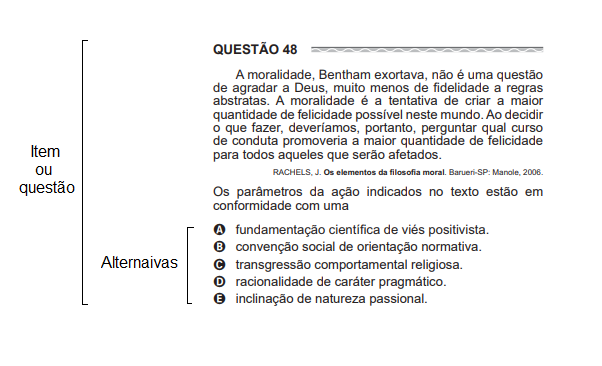
\includegraphics[width=0.5\linewidth]{img/ques.PNG}}\\
		Fonte: Questão 48 Enem 2017 / Primeiro Dia / Caderno azul .
		\label{fig:ques}
	\end{figure}
	\par
	    Assim o item é todo o conjunto: comando e as alternativas, sendo que uma das alternativas é a correta as as outras são apenas distratores, por isso diz-se itens dicotômicos(certo/errado). Quando um indivíduo endossa o item/questão diz-se que este acertou o item.
	 \par
		Um teste de múltipla consiste na escolha N itens ou questões, em geral, com 4 ou 5 alternativas de respostas, sendo uma, e somente uma, correta. O resultado é dado pelo número de acertos ou pelo percentual de acertos em uma escala própria de 0(zero) a 100 (cem), tomando como base a TCC(Teoria Clássica dos Testes). Em geral, não há julgamento sobre o que uma determinada nota significa, a não ser que notas acima de 70 costumam ser consideradas adequadas.\cite{Klein}
	
	\subsection{Teoria Clássica dos Testes(TCT)}
	\paragraph{}
	    Considerando um teste e seu escore Frederic Lord fez uma importante observação que o escore observado e o score verdadeiro de indivíduos examinados não tem o mesmo significado que a habilidade do indivíduo. Indivíduos podem ter baixos escores verdadeiros em um teste difícil e altos escores verdadeiros em um teste fácil, porém sua habilidade se mantém constante em relação qualquer outro teste que faça medição deste constructo. Claro que está habilidade esta sujeita à mudanças ao longo do tempo devido ao aprendizado posterior, porém no momento da aplicação do teste esta habilidade se mantém constante.
	\par
	    Lord e outros psicomotristas estavam interessados em um modelo que fossem independentes do conjunto de itens de um teste, No pensamento de Charles Spearman \cite{Spearman}, um dos fundadores da Teoria Clássica dos Testes, existiam erros nas medidas e que  erros eram variáveis aleatórias e que eles podiam ser correlacionados e classificados.
	\par
		Os testes de inteligência nas 4 primeiras décadas do seculo 20 levaram a criação da TCT\cite{Klein} muitos dos termos utilizados como score verdadeiro foi criada por Spearman's na sua teoria da inteligencia.
	\par
	    Segundo \textcite{Hamblenton} a TCT assume que cada pessoa tem um score verdadeiro, quando não há erros relacionados, o escore esperado para uma pessoa é dado por:
	 \par
	    \begin{equation}
	       X = T + E
	    \end{equation}
	\paragraph{}
	    Sendo que escore individual é o total de pontos em testes\cite{Ribeiro}.E $T$ o escore verdadeiro, $X$ o escore observado $X$ é o escore obtido por um estudante em um teste. E $E$ o erro relacionado.
	\par
	    Para cada indivíduo  existem duas incógnitas nesta equação, a é equação não pode ser resolvida a menos que algumas suposições sejam feitas.\cite{Klein}
	\paragraph{}
	\begin{enumerate}[label={\alph*)},noitemsep]
        \item escores verdadeiros e erro score são não correlacionados.
        \item a média do escore de erro na população de examinados é zero.
        \item o erro de score em testes paralelos(ver testes paralelos) são não correlacionados.
	\end{enumerate}
	\par
	   Por exemplo, Supondo que alguém saiba $70\%$ de um conteúdo este seria seu escore verdadeiro($T$), supondo existir um teste ideal ele mediria este escore, mas na realidade os testes medem um escore de $65\%$ a $75\%$ sendo que a discrepância de $5\%$ é o erro do escore.
	%$http://www.statisticshowto.com/classical-test-theory/$
    \par
    	No exemplo da tabela(\ref{tab:pessoas1}) exemplo, Pessoa 1 que respondeu todas as 5 itens corretamente, possui uma proficiência de $100\%$. \cite{Chong}. Entretanto não podemos julgar a proficiência de um indivíduo apenas com base no número de itens que este indivíduo acertou.
    \paragraph{}
    \begin{table}[!h]
    	\centering
    	\caption{Respostas de 5 pessoas a um teste hipotético}
    	\begin{tabular}{*{6}{c|}c}
    	    \hline
    	    resp & item 1& item 2& item 3 & item 4 & item 5 & score observado($X$)\\
    	    \hline
    	    \hline
    	     Pessoa 1 &  1 & 1 & 1 & 1 & 1 & 1\\
    	     Pessoa 2 &  1 & 1 & 1 & 1 & 0 & 0.8\\
    	     Pessoa 3 &  1 & 1 & 1 & 0 & 0 & 0.6\\
    	     Pessoa 4 &  1 & 1 & 0 & 0 & 0 & 0.4\\
             Pessoa 5 &  1 & 0 & 0 & 0 & 0 & 0.2\\
             Média &     1 & 0.8 & 0.6 & 0.3 & 0.2\\
             \hline
    	\end{tabular}
	    \label{tab:pessoas1}
	\end{table}
	\paragraph{}
		No exemplo da tabela(\ref{tab:pessoas2})em que a Pessoa 4 e a pessoa 6 tiveram o mesmo score, porém responderam itens diferentes, apesar de terem mesmo score não podemos afirmar nada sobre a proficiência de ambos os respondentes pois a pessoa 4 pode ter acertado itens fáceis enquanto a pessoa 6 acertado itens difíceis.
    \paragraph{}
	\begin{table}[!h]
	    \centering
	    \begin{tabular}{*{6}{c|}c}
	    \hline
	    respondente & item 1& item 2& item 3 & item 4 & item 5 & score observado($X$)\\
	    \hline
	    \hline
	        Pessoa 4 &  1 & 1 & 0 & 0 & 0 & 2\\
            Pessoa 5 &  1 & 0 & 0 & 0 & 0 & 1\\
            Pessoa 6 &  0 & 0 & 0 & 1 & 1 & 2 \\
            \hline
	    \end{tabular}
	    \caption{Respostas de 3 pessoas a um teste hipotético}
	    \label{tab:pessoas2}
	\end{table}
	\paragraph{}
		O quadro(\ref{tab:comparacao}) mostra as principais diferenças entre a TCT e a nova teoria que surgiria(TRI). E a TCT tinha também algumas limitações:
	\paragraph{}
    	\begin{enumerate}[noitemsep]
    	    \item As estatísticas que descrevem os itens de teste dependem do grupo de estudantes que fazem o teste.\\
            \item Os escores de teste que descrevem o desempenho dos alunos dependem dos itens apresentados aos alunos\\
            \item A Teoria Clássica dos Testes só pode ser utilizada em situações nas quais todos os alunos fazem o mesmo teste (ou formas “paralelas” de teste).\\
            \item A Teoria Clássica dos Testes não fornece um modelo do desempenho de um aluno em um item\\
            \item A maioria das aplicações da Teoria Clássica dos Testes assume incorretamente que os erros de medida têm a mesma variabilidade para todos os alunos. (Alguns aspectos da Teoria de Resposta ao Item relativos à estimação das proficiências)
	    \end{enumerate}
	\paragraph{}
	    Segundo \cite{Ronald} estas são as principais comparações entre TRI e TCT.
	\begin{table}[!h]
	    \centering
	    \caption{Comparação entre TCC e TRi}
	    \begin{tabular}{|p{4cm}|p{4cm}|p{4cm}|}
	        \hline
	         Área & TCT & TRI \\
	         \hline
	         \hline
	         Modelo & Linear & não-linear\\
	         \hline
	         Nível & Teste & Item \\
	         \hline
	         Habilidade item relação & Não especificado & CCI(curva caracteristica do item)\\
	         \hline
	         Invariancia entre item e a estatistica pessoal & Test scores or esti mated true scores are reported on the test-score scale (or a transformed test-score scale) & Ability scores are reported on the scale -00 to +00 (or a transformed scale)\\
	         \hline
	         Item statistics & p, r & b, a, and c (for the three-parameter model) plus corresponding item information functions \\
	         \hline
	         Sample size (for item parameter estimation) & 200 to 500 (in general) & Depends on the IRT model but larger samples, i.e., over 500, in general, are needed)\\
	         \hline
	    \end{tabular}
	     \label{tab:comparacao}
	\end{table}
	  
	\paragraph{}
	    Neste contexto A TRI foi desenvolvida principalmente para suprir limitações que a Teoria Clássica de Medidas /Teoria Clássica dos Testes(TCT) apresentava. dentre as quais se destaca que o instrumento de medida é dependente das características dos examinados que se submetem ao teste ou ao questionário.
	\par
	    Na TCT, a habilidade é medida da seguinte forma, o score total é a soma do número de questões corretas, na tentativa de estabelecer um nível de dificuldade ao teste, atribui-se pesos aos itens que compõem este teste. porém o modelo da TCT não consegue prever a coerência pedagógica e o “chute”.
	\par
	    A TRI tem uma abordagem diferente da TCT, o foco não está no teste e tratamos de probabilidades de de um individuo endossar um item, não tratamos de score e sim de habilidades. Porém a TRI não substitui a TCT.
	%(http://www.usf.edu.br/galeria/getImage/427/604207176923293.pdf)
		
	\newpage
	\subsection{Abordagem histórica}
	\paragraph{}
	    Segundo \textcite{Dalton} os primeiros modelos matemáticos que implementaram a TRI foram os dicotômicos, cujos possíveis resultados eram certo/errado ou concordo/descordo e outras variações de mesma natureza. Seja a resposta a um item $U_{ij} = 1$ para certo ou $U_{ij} = 0$ para item errado. Então surge a necessidade de encontrar uma função não linear que expressasse a probabilidade do respondente em função de sua habilidade dar uma resposta correta em função dos parâmetros do item. A própria necessidade desta função já impunha a restrição da CCI ser monótona crescente. %$https://www.maxwell.vrac.puc-rio.br/5253/5253\_4.PDF$
    \par	 
        Motivado pelo trabalho de \textcite{Lord}, Birnbaum fez uma modificação importante na teoria defendida por Lord, sugeriu a troca da função ogiva normal, proposta por Lord, pelo modelo logístico de dois parâmetros, por questões de conveniência. Além disso, foi Birnbaum, também, quem introduziu o terceiro parâmetro (vulgarmente conhecido como parâmetro de acerto casual, que modela um acerto em um teste educacional devido a um chute na questão)
	\par
		Como já foi dito, a TRI teve seus axiomas elaborados aos poucos desde os anos 50 por vários autores, embora suas raízes remontem há mais de uma década anterior. Entre estes precursores se encontram os trabalhos de Richardson (1936), comparando os parâmetros dos itens obtidos pela teoria clássica da Psicometria com os moldes que hoje usa a TRI. os trabalhos de Lawley (1943, 1944).
		Entretanto, o responsável mais direto que deu origem à TRI moderna, é Frederic Lord (1952, 1953).
		%http://pepsic.bvsalud.org/pdf/avp/v2n2/v2n2a02.pdf
	\par
        \textcite{Lord} foi o primeiro a desenvolver o modelo unidimensional de 2 parâmetros, baseado na distribuição normal. Após algumas aplicações desse modelo, o próprio Lord sentiu a necessidade da incorporação de um parâmetro que tratasse do problema do acerto casual. Assim, surgiu o modelo de 3 parâmetros. Anos mais tarde, \textcite{Birnbaum} substituiu, em ambos os modelos, a função ogiva normal pela função logística, matematicamente mais conveniente, pois é uma função explícita dos parâmetros do item e de habilidade e não envolve integração. Independentemente do trabalho de Lord, Rasch (1960) propôs o modelo unidimensional de 1 parâmetro, expresso também como modelo de ogiva normal e, também mais tarde descrito por um modelo logístico por Wright (1968).
        %teste
        \cite{Hamblenton}
	\subsection{Modelagem estatística da TRI}
	\paragraph{}
    	A TRI(Teoria de Resposta ao Item) é um conjunto de modelos estatísticos-matemáticos que procuram representar a probabilidade de um indivíduo dar uma resposta correta a um item como função dos parâmetros deste item e da habilidade (ou habilidades) do respondente. Essa relação é sempre expressa de tal forma que quanto maior a habilidade, maior a probabilidade de acerto no item, figura(). Segundo \textcite{Dalton}, os vários modelos propostos na literatura dependem fundamentalmente de três fatores:\\
    	\begin{enumerate}
    	    \item da natureza do item | dicotômicos(Figura 1) ou politômicos(Figura 2);
    	    \item do número de populações envolvidas | apenas uma ou mais de uma;
    	    \item da quantidade de traços latentes que está sendo medida | apenas um(modelo unidimensional) ou mais de um.
    	\end{enumerate}
    \paragraph{}
    	Entende-se por natureza dicotômica itens que aceitem certo/errado ou concordo/descordo como possíveis respostas, e itens politômicos sendo itens que contenham mais de três opções de respostas certo/errado/meio certo pu nenhum pouco/só um pouco/bastante/demais. Uma questão politômica pode ser observada no questionário  SNAP, questionário  para levantamento de alguns  possíveis  sintomas  primários  do  TDAH, como pode ser observado neste item:
    \newpage
	\begin{enumerate}
	    \item[H1] Não consegue prestar muita atenção a detalhes ou comete erros por descuido nos trabalhos da escola ou tarefas.
	    \begin{enumerate}
	        \item nenhum pouco
	        \item só um pouco
	        \item bastante
	        \item demias
	    \end{enumerate}
	\end{enumerate}
\par
	    A escolha da população fica a critério do pesquisador/avaliador, exemplo: podemos numa escola que tenham duas turmas de 5º ano, uma diurna outra noturna podemos fazer a escolha da população considerando apenas o 5º ano como uma população ou duas populações 5º ano A e 5º ano B. %O Enem utiliza
	\par
    	Explicam que o modelo de Rasch tem como uma de suas características fundamentais a premissa de que o comportamento de um. sujeito frente a um item pode ser explicado em função das características ou das atitudes
    	latentes $(\theta)$, que não são observadas diretamente. Nesse sentido, a variável latente de um
    	sujeito, o traço, influi sobre a probabilidade de acertar um item específico.
	 \par
	 	Quanto a quantidade de traços latentes trata-se do conceito muito importante para a escolha de qual modelo implementar. Quando estamos interessado em medir apenas um traço latente temos que utilizar modelos unidimensionais, caso contrario buscamos os modelos multidimensionais.
	 \par 
	    Busca-se através do modelo da unidimensionalidade encontrar apenas uma habilidade responsável por todas as outras habilidades. Sabemos que as atividades humanas requerem múltiplas habilidades para que uma determinada tarefa seja executada,  para a habilidade ou proficiência de um indivíduo não é diferente, um item para ser respondido corretamente necessita de diversas habilidades. Então para que haja a unidimensionalidade é necessário supor que existe uma habilidade responsável pelas demais habilidades necessárias para o endosso ao item. Porém existem modelos que supõem que mais de uma habilidade está sendo medida, os chamados modelos multidimensionais.
	 \par
		Traços latentes são características do indivíduo que não podem ser medidas diretamente, ou seja, não existe um aparelho capaz de medi-las diretamente, como nível de ansiedade, nível de depressão, proficiência, níveis de uma determinada emoção etc. Portanto, essas características são mensuradas através de variáveis secundárias que sejam relacionadas com o traço latente em estudo. Na busca por instrumentos que medissem traços latentes, a psicometria responsável pela junção da psicologia com as ciências exatas, apoderou-se de uma gama de modelos estatísticos que busquem estimadores para do parâmetro a ser medido.
	\par
	    Um traço latente deve ser inferido a partir da observação de variáveis secundárias que estejam relacionadas a ela, ou seja, a resposta do indivíduo. As características ocultas são difíceis de serem quantizadas por se tratarem de quantidades subjetivas.\\ 
	\par
	    os traços latentes se diferem de outras medidas por não poderem ser medidas por instrumentos físicos, por exemplo a massa e a temperatura que podem ser medidas por uma balança e termômetro.
	\par
	    Assim, se um pesquisador deseja obter a medida de um determinado traço latente, ele deve caracterizar a natureza do traço latente a ser medido, construir os itens que devem cobrir todo o traço latente, observar o tipo de resposta que é dado ao item para verificar se os itens têm natureza acumulativa ou de desdobramento e, a partir daí, escolher o modelo da TRI mais adequado que se ajuste ao seus dados. Em seguida, estimar os parâmetros dos itens e dos respondentes e construir e interpretar a escala do traço latente.
	\par
	    No âmbito da avaliação educacional a habilidade/proficiência de um aluno/respondente é o  traço latente no qual busca-se estimar. No entanto a função para o estimador da  habilidade de um respondente, não pode ser tida como uma função linear, ou seja, não é necessariamente verdade que a probabilidade de um aluno dar uma resposta correta a um item seja diretamente proporcional a sua habilidade. Por isso  A TRI(Teoria de Resposta ao item) surge como um conjunto de modelos matemáticos  que teve seus princípios básicos estabelecidos nos anos 1960, tomando conta de grande parte da psicometria nos anos 1980. Estas teorias postulam que o comportamento humano é consequência de processos hipotéticos chamados de traços latentes. Assim indivíduos com baixa habilidade tem baixa probabilidade de acertar o item e indivíduos com alta habilidade tem alta probabilidade de acertar o item.O modelo expressa a relação entre os comportamentos que são as respostas dadas aos itens as chamadas variáveis observáveis e os traços latentes (as variáveis hipotéticas) através uma equação matemática chamada de equação logística. Esta produz uma curva ou ogiva conhecida como a curva característica do item, a CCI. A CCI define os parâmetros dos comportamentos, ditos itens (dificuldade, discriminação e acerto casual) em função do tamanho do traço latente, expresso como teta $\theta$.\cite{Pasquali}
	\par
    	Neste trabalho utiliza-se para referência ,modelos que envolvem uma única população, o modelo logístico de 3 parâmetros e o modelo dicotômico, assim o modelo matemático utilizado será: modelo logístico unidimensional de 3 parâmetros (ML3). Sendo que o ML1 e ML2 podem ser obtidos a partir do ML3.
    	
    	%http://georgek.people.uic.edu/Karabatsos.pdf
    	
    \newpage
    	\noindent Definição função logística para o estimador:\\
	\begin{equation}
		P_i(U_{ij} = 1,\theta_j) = c_i + (1-ci)\displaystyle\frac{1}{1 + e^{-Da_i(\theta_j - b_i)}}
	\end{equation}
	    Onde:\\
	\begin{enumerate}[noitemsep]
	    \item[]  $0 < P_i < 1$ é a probabilidade de um respondente j com uma habilidade $\theta$ responder corretamente um item i com dificuldade b.
	    \item[] O parâmetro $b_i$  representa a dificuldade do   item i.
	    \item[] O parâmetro $a_i$ representa a discriminação do item i.
	    \item[] O parâmetro $c_i$ representa a probabilidade de um a um respondente com baixa habilidade responder corretamente ao item,  também conhecido como parâmetro de “chute”.
	    \item[] $\theta_j$ representa  a habilidade do respondente j.
	    \item[] $e$ é a constante $2.7182...$, conhecido como Número de Euler.
    	\item[] $D$  é uma constante $1.7$ para se aproximar de uma curva de ogiva normal. 
	\end{enumerate}
	\paragraph{}
    	O parâmetro de dificuldade($b$) que está na mesma escala que a habilidade($\theta$) refere-se a habilidade miníma para um indivíduo responder corretamente a um item. Em outras palavras é o valor no qual $P(U_i = 1, \theta)  = 0.5$
    \par
	    O parâmetro de discriminação é a capacidade que um item tem de distinguir os indivíduos que têm a proficiência requisitada daqueles quem não a têm. É também um valor no qual a derivada de $P(U_i = 1, \theta )$  no ponto em que $b = \theta$, graficamente podemos ver na figura(\ref{fig:Rplo2}) que quanto maior o declive da curva para habilidades próximas a dificuldade do item podemos ter uma discrepância grandes nas probabilidades,ou seja, este  item discrimina quem sabe e quem não sabe.
	\paragraph{}
	\begin{figure}[!h]
	    \centering
	    \caption{Curva característica do item}
	    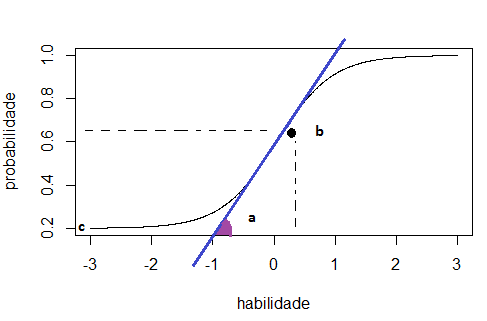
\includegraphics[width=0.48\linewidth]{img/Rplo2}\\
	    Fonte: Autor
	    \label{fig:Rplo2}
	\end{figure}
	\paragraph{}
    	\noindent A equivalência entre modelos ocorre quando:\\
    	O parâmetro de chute $c_i$ é igual a $0$ para todos os itens, que é equivalente ao modelo logístico de 2 parâmetros:
    \paragraph{}
	\begin{eqnarray}
		P_i(U_{ij} = 1,\theta_j) & = & c_i + (1-ci)\displaystyle\frac{1}{1 + e^{-Da_i(\theta_j - b_i)}} | c_i - 0 \nonumber \\ 
		P_i(U_{ij} = 1,\theta_j) & = & 0 + (1-0)\displaystyle\frac{1}{1 + e^{-Da_i(\theta_j - b_i)}} \nonumber \\
		P_i(U_{ij} = 1,\theta_j) & = & \displaystyle\frac{1}{1 + e^{-Da_i(\theta_j - b_i)}} \nonumber
	\end{eqnarray}
    	
    	\
    \noindent O parâmetro de chute é 0 e o parâmetro de discriminação é 1 sendo equivalente ao modelo logístico de 1 parâmetro\\
	
	\begin{eqnarray}
		P_i(U_{ij} = 1,\theta_j) & = & c_i + (1-ci)\displaystyle\frac{1}{1 + e^{-Da_i(\theta_j - b_i)}} | c_i - 0 | a_i = 1\\
		P_i(U_{ij} = 1,\theta_j) & = & 0 + (1-0)\displaystyle\frac{1}{1 + e^{-D*1*(\theta_j - b_i)}} \\
		P_i(U_{ij} = 1,\theta_j) & = & \displaystyle\frac{1}{1 + e^{-D*1*(\theta_j - b_i)}}
	\end{eqnarray}
    	
    \subsection{Modelo de Rasch}
    \paragraph{}
    	Rasch desenvolveu seu modelo independentemente da TRi, Sendo frequentemente considerado com o parametro de 1 parametro o modelo de Rasch apesar de alguns autores dierem ser uma bordagem totalmente diferente quanto aos conceitos.

	
\subsection{Curva característica do item}
    \paragraph{}
		Na definição moderna da TRI cada um dos itens terá uma curva característica(CCI), Segundo \cite{Baker}, Terman ainda na Teoria clássica dos testes, em 1916 Termam utilizando os dados das observações de Binet plotou a proporção de respostas corretas como função da idade cronológica na escala de inteligência de Binet-Simon, e traçou uma linha entre os pontos criando assim a CCI(\ref{fig:cci_age}). Binet colocou no teste de inteligencia um item cuja proporção de respostas corretas dadas pelos respondentes era de 0,75 , no caso da figura, mas qualquer outra proporção poderia ser usada, Termam utilizou a proporção 0,50. SendoTucker foi primeiro a utilizar a expressão curva característica do item.
	\begin{figure}[!h]
	    \centering
	    \caption{Plote de idade cronológica}
	    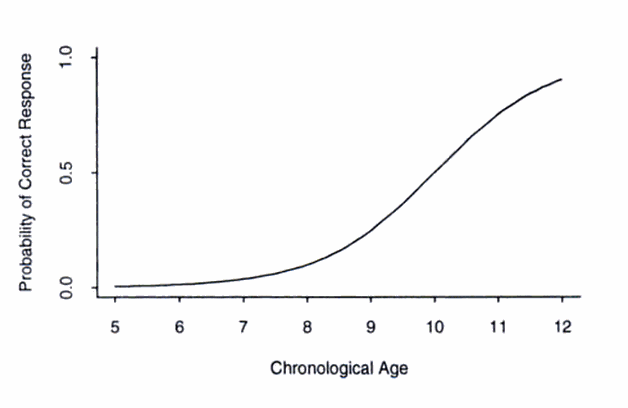
\includegraphics[width=0.5\linewidth]{img/age}
	    \label{fig:cci_age}
	\end{figure}
	   
	\paragraph{}
    	Assim podemos ver que a curva característica é a relação entre a proporção de respostas corretas ao item e uma variável de interesse, no caso de Binet a inteligência, na avaliação escolar a habilidade ou proficiência.
    \paragraph{}
    
    
    
        Os modelos dos modelos  curva características do item existentes, apenas dois são os mais utilizados: o modelo de ogiva normal e o modelo logístico normal. Muitas outras funções fora dessa classe foram propostas, tal como a função linear, mas com pouco efeito prático e sérias limitações nos valores possíveis para as habilidades(\cite{Ribeiro}).
    \subsubsection{Curva ogiva normal}
    \begin{figure}[!h]
    	\centering
    	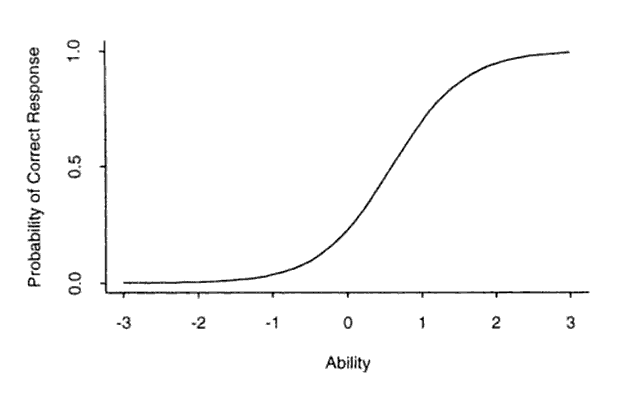
\includegraphics[width=0.6\linewidth]{img/ogiva}
    	\caption{}
    	\label{fig:ogiva}
    \end{figure}
    \paragraph{}
        Modelo proposto por Lord:
    \begin{equation}
        P(\theta) = \displaystyle\int_{-\infty}^{a_i(\theta - b_i)}\displaystyle\frac{1}{\sqrt{2\pi}}e^{-t^2/2}dt
    \end{equation}
    \paragraph{}
        Pode ser entendido de acordo com dois pontos de vista, Segundo (tem Response Theory: Parameter Estimation Techniques, Second Edition) autores como Richardson e Ferguson e Finney  simplesmente assumindo que a curva característica do item pode ser modelado por uma ogiva normal, fazendo teste e comparando as proporções de respostas corretas assim a ogiva normal provou-se se adaptar aos dados. a segunda explicação é dada por \cite{Novick} mais teórica.
        
    \subsubsection{Curva logística}
    \begin{figure}[!h]
    	\centering
    	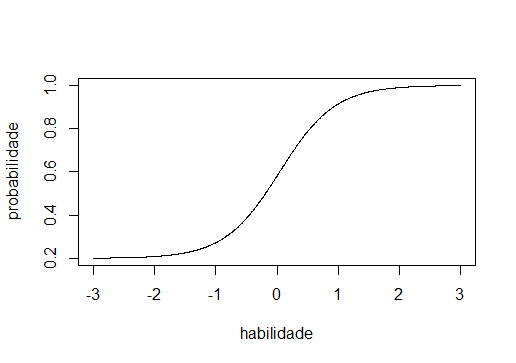
\includegraphics[width=0.6\linewidth]{img/Rplo}
    	\caption{}
    	\label{fig:rplo}
    \end{figure}
    \paragraph{}
        Muito similar ao modelo de ogiva normal, o segundo modelo, utilizado pela tri é o modelo logístico sendo atribuído a Birnbaum este modelo é também utilizado para o crescimento da população, plantas, pessoas. Segundo \cite{Baker} ambos modelos são usado em tri porem o modelo logístico é predominante na literatura acadêmica.
    \paragraph{}
        A forma da função logística:
    \begin{equation}
        P_i(\theta) = \displaystyle\frac{e^{Z_i}}{1 + e^{Z_i}} = \displaystyle\frac{1}{1 + e^{-Z_i}}
    \end{equation}
    
    Onde:\\
    $Z_i = a_i(\theta - b_i)$, também chamado de logit. 
    \paragraph{}
        O modelo de ogiva normal foi usado nos anos 1960, porem devido a demanda computacional que este modelo exigia foi preterido em relação ao modelo logístico. entretanto atualmente devido ao avanço dos computadores e com o de series polinomiais para funções de ogiva normal.
	\subsection{Conceitos Estatísticos}
    	Para melhor entendimento buscamos uma definição no livro \cite{Sonia}
	 \begin{enumerate}
	 	\item[]  \textbf{População} É uma coleção completa de todos os elementos a serem estudados.
	 	\item[] \textbf{Amostra} É uma subcoleção de elementos extraídos de uma população.
	 	\item[] \textbf{Parâmetro} É uma medida numérica que descreve uma característica de uma população.
	 	 \item[] \textbf{Estatística} É uma medida numérica que descreve uma característica de uma amostra.
	 	 \item[] \textbf{Estimador} É um regra para calcular uma estimativa de uma determinada quantidade baseada em dados observados.
	\end{enumerate}
	\paragraph{}
	    No âmbito da avaliação educacional a TRI  que procuram representar a probabilidade de um indivíduo dar uma certa resposta a um item como função dos parâmetros do item e da habilidade (ou habilidades) do respondente. Essa relação é sempre expressa de tal forma que quanto maior a habilidade, maior a probabilidade de acerto no item. Os vários modelos propostos na literatura dependem fundamentalmente de três fatores, está definição e da Tri voltada para a avaliação educacional.

	\newpage